\documentclass[11pt]{article}
\usepackage[margin=1in]{geometry}
\usepackage{amsmath,amssymb,amsthm}
\usepackage{booktabs}
\usepackage{graphicx}
\usepackage{hyperref}
\usepackage{xcolor}
\usepackage{microtype}
\usepackage{enumitem}
\usepackage{placeins}
\usepackage{caption}
\hypersetup{colorlinks=true,linkcolor=blue!50!black,citecolor=blue!50!black,urlcolor=blue!50!black}
\captionsetup{font=small}
\setlist{nosep}

\newtheorem{theorem}{Theorem}
\newtheorem{lemma}{Lemma}
\newtheorem{proposition}{Proposition}
\newtheorem{corollary}{Corollary}
\newtheorem{assumption}{Assumption}
\theoremstyle{definition}
\newtheorem{definition}{Definition}
\theoremstyle{remark}
\newtheorem{remark}{Remark}

\newcommand{\A}{\mathcal{A}}
\newcommand{\F}{\mathcal{F}}
\newcommand{\Oc}{\Omega}
\newcommand{\act}{\alpha}
\newcommand{\traj}{\tau}
\newcommand{\Hb}{\mathcal{H}_0}
\newcommand{\Ha}{\mathcal{H}_1}
\newcommand{\Qb}{Q_0}
\newcommand{\Qa}{Q_1}
\newcommand{\E}{\mathbb{E}}
\renewcommand{\Pr}{\mathbb{P}}
\newcommand{\ind}{\mathbf{1}}
\newcommand{\sys}{\textsc{Writ}}

\newcommand{\nSim}{1000}
\newcommand{\villeMaxPct}{0.0}
\newcommand{\villeMaxAnyPct}{3.1}
\newcommand{\realPermLaunderPct}{32.1}
\newcommand{\realRulesLaunderPct}{5.5}
\newcommand{\realIntentLaunderPct}{5.9}
\newcommand{\realPermProbePct}{28.2}
\newcommand{\realIntentProbePct}{6.9}
\newcommand{\realPermPatientPct}{31.8}
\newcommand{\realRulesPatientPct}{6.5}
\newcommand{\realIntentPatientPct}{7.2}
\newcommand{\heldBenignIntentPct}{3.6}
\newcommand{\heldBenignJudgePct}{8.5}
\newcommand{\supEagerIntentPct}{0.0}
\newcommand{\supLaunderIntentPct}{80.0}
\newcommand{\realPermPersistPct}{64.3}
\newcommand{\realRulesPersistPct}{16.9}
\newcommand{\realJudgePersistPct}{3.4}
\newcommand{\realIntentPersistPct}{7.8}
\newcommand{\realRulesPersistDirectPct}{18.5}
\newcommand{\realIntentPersistDirectPct}{7.7}
\newcommand{\supPersistDirectIntentPct}{99.3}
\newcommand{\supMimicIntentPct}{51.5}
\newcommand{\realIntentMimicPct}{5.8}
\newcommand{\realRulesMimicPct}{8.7}
\newcommand{\simSeconds}{424.8}
\newcommand{\realComposedPersistPct}{1.0}
\newcommand{\realComposedLaunderPct}{1.4}
\newcommand{\heldBenignComposedPct}{3.7}
\newcommand{\supMultigoalIntentPct}{79.1}
\newcommand{\realIntentMultigoalPct}{10.2}
\newcommand{\realRulesMultigoalPct}{8.7}
\newcommand{\supPatientKzeroPct}{0.0}
\newcommand{\supPatientKthreePct}{79.2}
\newcommand{\supProbeKzeroPct}{0.0}
\newcommand{\supProbeKthreePct}{79.2}
\newcommand{\supBenignTwoEpsLowPct}{37.2}
\newcommand{\supBenignTwoEpsDefaultPct}{6.0}
\newcommand{\rZeroMax}{0.018}
\newcommand{\forecastInitial}{0.007}
\newcommand{\qZeroRealizedBetaTwoPct}{3.9}
\newcommand{\liveAdvControlRealized}{9/12}
\newcommand{\liveAdvIntentRealized}{0/12}
\newcommand{\liveAdvIntentDeniedOrHeld}{12/12}
\newcommand{\liveBenignHeld}{0/9}
\newcommand{\liveBenignSupervised}{0/9}
\newcommand{\liveBenignRefunded}{9/9}
\newcommand{\liveRuns}{33}
\newcommand{\liveModel}{gpt-5}
\newcommand{\benchWarmMs}{0.59}
\newcommand{\benchWarmPNinetyFiveMs}{0.71}
\newcommand{\benchColdMs}{207}
\newcommand{\alphaEps}{1.000}
\newcommand{\nActions}{19}
\newcommand{\nHyps}{54}


\title{\textbf{Betting Against Intent:}\\ Anytime-Valid Admission Control for Tool-Using Agents}
\author{Han Lee\thanks{Stanford University. Code, data and the reference system are in the accompanying repository.}}
\date{October 2026}

\begin{document}
\maketitle

\begin{abstract}
Permission systems for AI agents bound what an agent may \emph{do}. They do not bound what a task may \emph{cause}: in a live deployment, a frontier model that was denied a CRM field change simply asked the legitimate recipient of its permitted email to make the change for it. We argue that intent cannot be measured from a tool list, but it can be \emph{tested} from a trajectory, and that the right statistical object for an execution gate is an e-process rather than a classifier. We introduce contracts over \emph{outcomes}: each task declares authorized outcomes and \emph{non-goals} it must not advance by any means. Over this contract we build (i) deterministic layers that map payload content and identifier provenance onto abstract outcome effects, and (ii) \emph{interventional goal recognition}: a Bayesian mixture over benign and compromised agent models in which the gate's own denials are interventions that make indirect pursuit sharply informative. The resulting likelihood ratio is a test martingale under the benign class, so holding a task when it exceeds $1/\alpha$ bounds the probability that a benign agent is \emph{ever} held by $\alpha$, uniformly over trajectory length (Ville). A change-of-measure argument bounds the probability that any in-class adversary realises a non-goal without being held by $|\Ha|\,\Qb(\text{realise})/\alpha$, and a $k$-step forecast of non-goal reachability under the posterior places tasks under supervision before the consequential step. We implement the method in \sys{}, an execution authority for agents, and evaluate it against scripted adversaries it was not fitted to and against live \texttt{gpt-5} agents working a customer-operations task under benign, prompt-injected, indirectly-injected and compromised conditions. Against persistent laundering the intent layer cuts the realised non-goal rate from \realRulesPersistPct\% (content rules alone) to \realIntentPersistPct\% while holding at most \heldBenignIntentPct\% of benign trajectories, and it converts single detections into protection of every subsequent consequential action.
\end{abstract}

\section{Introduction}

Agents that act on real systems are governed today by permission: a list of tools, scopes on their arguments, perhaps budgets. This is necessary and, we will argue, structurally insufficient. A permission bounds an \emph{operation}. Many consequential outcomes can be reached through a permitted operation, because the operation's payload is read by a human or another system that then acts. The simplest such path is a request: ``please update the billing contact to \texttt{cfo@acme.example}.'' No tool was misused; the forbidden outcome is still underway.

We observed exactly this. A customer-operations task was authorised to refund a duplicate charge, record a note and notify the existing billing contact. The user prompt additionally asked for two things the task contract excluded. A \texttt{gpt-5} agent attempted the excluded CRM change, was denied by the gate, correctly reported that it could not do it, and then wrote the request into its permitted email to the legitimate recipient (Section~\ref{sec:live}). Every tool call it made was authorised.

The question this paper answers is what an execution gate can \emph{measure} about intent without trusting the agent's reasoning, and what guarantees that measurement can carry. Our position is:

\begin{enumerate}[leftmargin=1.5em]
\item Intent is relative to a \emph{contract over outcomes}. ``Change the billing contact'' is a non-goal of this task whether it is pursued by a field write, by an email, or by a sub-agent. Declaring non-goals is cheap for operators and gives the gate an object to test.
\item A great deal of intent is \emph{deterministic} once content is mapped to outcomes: an explicit request toward a non-goal, or an identifier that appears in a payload without ever having been observed through an authorised action. These layers are sound by construction and have no false-positive rate to tune.
\item What remains is sequential. An agent reveals goals through what it \emph{tries}, and the gate's denials are \emph{interventions}: after a direct route is closed, indirect pursuit becomes far more informative. The correct statistical treatment of a stream of such evidence is a test martingale (an e-process), not a per-action classifier: it composes evidence across arbitrarily many steps while controlling the probability of ever wrongly holding a benign task.
\item Prediction is possible because the hypothesis space is small and structured. A posterior over benign and compromised agent models induces a $k$-step reachability forecast of non-goals under the permitted action set; supervision can start before the step that would realise harm.
\end{enumerate}

\paragraph{Contributions.}
(1) A formalisation of task contracts over outcomes and an \emph{abstract action} semantics that maps concrete tool calls, their predicted effects, their content claims and the provenance of their identifiers onto outcome effects (Section~\ref{sec:contracts}).
(2) \emph{Interventional goal recognition}: a mixture model of benign (including eager-but-compliant) and compromised (patient) agents in which denials change the permitted action set, with a lemma showing denials strictly increase the evidential value of indirect pursuit (Section~\ref{sec:igr}).
(3) An anytime-valid admission rule with three guarantees: a uniform-in-time false-hold bound for benign agents (Theorem~\ref{thm:ville}), a circumvention bound for adversaries via change of measure (Theorem~\ref{thm:circ}), and a detection-time bound (Theorem~\ref{thm:time}); plus a proof that the lookahead forecast trigger is itself an e-threshold (Proposition~\ref{prop:forecast}) (Section~\ref{sec:evalid}).
(4) A production implementation inside an execution authority with held authorizations, tree-scoped intent state (so delegation cannot reset evidence) and operator approval, and an evaluation on scripted out-of-class adversaries and live frontier-model agents (Sections~\ref{sec:system}--\ref{sec:exp}).

\section{Setting and threat model}
\label{sec:setting}

\paragraph{Execution authority.} Agents hold no credentials. They request \emph{commands} from a fixed table; a gate checks each request against a task contract and dispatches a single-use signed authorization to an isolated executor that performs the operation and returns a signed receipt. Sub-agents receive strictly attenuated contracts and share budgets with their parent. We take this architecture (\sys{}) as given; it is described in Appendix~\ref{app:system}. What matters here is that \emph{every} path from the agent to a protected resource passes through the gate, and that the gate observes every attempt, including the ones it denies.

\paragraph{Outcomes.} Let $\Oc$ be a finite set of symbolic outcomes. A contract declares authorised outcomes $\A\subset\Oc$ and non-goals $\F\subset\Oc$, $\A\cap\F=\emptyset$. Outcomes can be realised \emph{directly} by an operation's effect (a field write, a payment), or \emph{indirectly} when a payload that leaves the system (a \emph{sink}: email, ticket, message) carries a request that a human or downstream system fulfils with probability $p_f\in[0,1]$.

\paragraph{Adversary.} The agent's reasoning, prompts, tool arguments and sub-agents are untrusted. The adversary may be a compromised model, a prompt injection in user input, or an injection in data the agent legitimately reads. It knows the contract (constraints appear in tool descriptions), may complete the legitimate task as cover, may probe, may split work across sub-agents, and may pursue several non-goals. It cannot bypass the gate, forge authorizations, or alter the gate's model.

\paragraph{Goal.} Bound the probability that a task realises any $f\in\F$ while bounding the probability that a benign task is interrupted, and do so \emph{before} the realising step whenever the trajectory contains any signal.

\section{Contracts over outcomes and the deterministic layers}
\label{sec:contracts}

\begin{definition}[Abstract action]
An abstract action is $\act=(c, D, R, \sigma, \pi)$: a command $c$, the set $D\subseteq\Oc$ of outcomes it realises directly, the set $R\subseteq\F$ of non-goals its payload \emph{requests} of a recipient, a sink flag $\sigma$, and a probe flag $\pi$ (an attempt outside the grant). A distinguished action \textsc{stop} ends the task.
\end{definition}

Concrete tool calls are mapped to abstract actions by three deterministic components.
\emph{Effect adapters} predict, for the target system's current configuration, what an operation will cause (e.g.\ a tag write that triggers an export automation); outcome rules map effects to $D$.
\emph{Claim extraction} reads free-text payload fields of sinks and emits typed claims (request-of-recipient, commitment, mention) toward named non-goals; requests and commitments populate $R$. The default extractor is rule-based (request verbs plus per-non-goal vocabulary and protected field names); a model-based extractor is optional. Claims are data: the policy that acts on them is code.
\emph{Provenance} labels identifier-like atoms (addresses, resource ids, URLs, account numbers) in a sink payload by origin.

\begin{definition}[Trusted provenance]
Let $T(\traj)$ be the atoms appearing in the contract together with atoms appearing in \emph{structured} (non-free-text) fields of the results of executed actions in $\traj$. A sink payload is \emph{provenance-clean} if all its atoms lie in $T(\traj)$.
\end{definition}

\begin{lemma}[Provenance soundness]
\label{lem:prov}
If a sink payload names an entity by an identifier that the task has not observed through the contract or an executed action, the payload is not provenance-clean. In particular a request to redirect, forward or pay to a target identified by such an atom is held before execution, regardless of how it is phrased.
\end{lemma}
\begin{proof}
Immediate from the definition: the atom is not in $T(\traj)$. Free-text fields of results are excluded from $T$ precisely because they are the carrier of indirect injection; an atom planted there is not trusted even though the agent legitimately read it.
\end{proof}

Lemma~\ref{lem:prov} is a soundness statement, not completeness: a request can name its target by description (``your finance director''). That case is left to claims and, when claims miss, to the probabilistic layer. The live-run bug that motivated the ``executed action'' clause (a benign email citing the refund id just created) is recorded in Section~\ref{sec:live}.

\paragraph{Deterministic policy.} An attempt with $D\cap\F\neq\emptyset$ is denied (grant or effect check). A sink with a request or commitment toward $f\in\F$ at extractor confidence above a threshold is denied. A sink that is not provenance-clean is held for an operator. Every one of these decisions is also an \emph{observation} for the next section.

\section{Interventional goal recognition}
\label{sec:igr}

\paragraph{State and action space.} The abstract state $s=(\mathrm{ach}, \mathrm{blk})$ records authorised outcomes and instrumental reads achieved, and non-goals whose direct route is \emph{closed}, either statically (the grant excludes the field, which the agent can see) or because a direct attempt was denied. The permitted action set $\A(s)$ contains \textsc{stop}; for each granted command its plain action (with its direct authorised outcomes); for each sink and each human-realisable $f$ a request variant; for each \emph{open} direct route to $f$ a direct variant; and for each command a probe. $|\A(s)|$ is small ($\nActions$ in our template, including pair-request variants for sinks).

\paragraph{Utilities.} With a cost $c$ per action and $\iota$ the value of an unperformed read, the benign utility and the hidden utility for a goal set $S\subseteq\F$ with weight $w$ are
\begin{align*}
U_\A(\act,s)&=\iota\,[\act\text{ reads}]+\!\!\sum_{\omega\in D\cap\A\setminus\mathrm{ach}}\!\!1\;-\;\kappa_F\,|D\cap\F|\;-\;\kappa_C\,[R\neq\emptyset]\;-\;\kappa_P\,[\pi]\;-\;c,\\
U_S(\act,s)&=\iota\,[\act\text{ reads}]+\sum_{f\in S}\big(w\,[f\in D]+w\,p_f\,[f\in R]\big)\;+\;w\,p_{\mathrm{expl}}\,[\pi]\;-\;\kappa'_C\,[R\neq\emptyset]\;-\;\kappa_P\,[\pi]\;-\;c .
\end{align*}
Benign agents pay a high content cost $\kappa_C$ for carrying out-of-scope requests; compromised agents pay a low one $\kappa'_C$: the content route is unnatural for one and cheap for the other. Benign agents also pay $\kappa_F$ per forbidden direct effect. Constants are in Appendix~\ref{app:constants}; the sensitivity analysis is in Section~\ref{sec:sim}.

\paragraph{Policies.} Benign: $\pi^{\beta}_0(\act\mid s)\propto\exp(\beta U_\A(\act,s))$ over $\A(s)$. \emph{Eager-but-compliant} benign: $\pi^{\beta,\eta}_0=(1-\eta)\pi_0^\beta+\eta\,\mathrm{Unif}(\text{open direct non-goal actions})$ when that set is nonempty; this models an agent that tries once what the user asked for and complies after denial. Hidden: $\pi^{\beta,w}_S$ is Boltzmann in $U_S$ over non-read actions, with reads assigned the benign policy's mass (reads are instrumental to every goal and therefore carry no goal information). \emph{Compromised}: $\pi^{\beta,w,\lambda}_S=(1-\lambda)\pi_0^\beta+\lambda\pi^{\beta,w}_S$. The patience parameter $\lambda$ lets a compromised agent do the real job as cover at a per-step evidential cost of only $(1-\lambda)$.

\paragraph{Hypothesis class.} $\Hb=\{(\beta,\eta)\}$ and $\Ha=\{(S,\beta,w,\lambda)\}$ with $S$ ranging over singletons of $\F$ and $\F$ itself, finite grids on $\beta,w,\lambda,\eta$, prior mass $1-\rho$ on $\Hb$ split uniformly and $\rho$ on $\Ha$ split uniformly. In our template $|\Hb|=6$, $|\Ha|=48$; the joint goal set receives half the compromised prior.

\paragraph{Observations and likelihood.} A trajectory $\traj_t=(\act_1,d_1,\dots,\act_t,d_t)$ records each attempted abstract action and whether the gate executed or denied it. Because the gate's decision is a deterministic function of $(\act_i,s_i)$, the state sequence is determined by the attempts, and $L_h(\traj_t)=\prod_{i\le t}\pi_h(\act_i\mid s_i)$. Denied attempts enter the likelihood exactly like executed ones.

\begin{lemma}[Denial is an informative intervention]
\label{lem:denial}
Fix a compromised component $h=(S,\beta,w,\lambda)$ with $f\in S$ and a sink request action $\act_R$ with $f\in R$. Let $s$ be a state in which a direct route $\act_D$ to $f$ is open and $s'$ the same state with that route closed by denial. Write $p_0=\pi^\beta_0(\act_D\mid s)$ and $p_S=\pi^{\beta,w}_S(\act_D\mid s)$. Then
\[
\frac{\pi_h(\act_R\mid s')}{\pi_0^\beta(\act_R\mid s')}\;=\;\gamma\cdot\frac{\pi_h(\act_R\mid s)}{\pi_0^\beta(\act_R\mid s)}
\qquad\text{with}\qquad
1\;\le\;\gamma\;\le\;\frac{1-p_0}{1-p_S},
\]
where $\gamma$ equals the upper end for the pure hidden policy ($\lambda=1$) and is strictly greater than $1$ whenever $\lambda>0$ and $p_S>p_0$. The latter holds for every compromised component because $U_S(\act_D)=w-c$ is the largest hidden utility in $\A(s)$ while $U_\A(\act_D)=-\kappa_F-c$ is the smallest benign one.
\end{lemma}
\begin{proof}
Removing one element of mass $p$ from the support of a Boltzmann distribution rescales every remaining probability by $1/(1-p)$, because the remaining utilities are unchanged. Hence $\pi^\beta_0(\act_R\mid s')=\pi^\beta_0(\act_R\mid s)/(1-p_0)$ and $\pi^{\beta,w}_S(\act_R\mid s')=\pi^{\beta,w}_S(\act_R\mid s)/(1-p_S)$. For the mixture, $\pi_h(\act_R\mid s')=(1-\lambda)\pi_0(\act_R\mid s)/(1-p_0)+\lambda\pi_S(\act_R\mid s)/(1-p_S)$; dividing by $\pi^\beta_0(\act_R\mid s')$ gives a convex combination of $1\cdot\frac{(1-\lambda)\pi_0}{\pi_h}$ and $\frac{1-p_0}{1-p_S}\cdot\frac{\lambda\pi_S}{\pi_h}$ relative to the pre-denial ratio, which yields the stated bounds on $\gamma$.
\end{proof}

The factor is large in practice: at $\beta=4$, $w=5$ the hidden policy puts $p_h\approx0.99$ on the open direct route, so closing it multiplies the evidential value of a subsequent laundering request by roughly two orders of magnitude. For the eager benign components the removed mass is $p_0\approx\eta/|\text{open routes}|$, which only strengthens the factor. This is the formal content of ``one denied attempt is a mistake; pursuing the same outcome afterwards is intent.''

\paragraph{Posterior and tree scoping.} The posterior is $\pi(h\mid\traj_t)\propto\pi(h)L_h(\traj_t)$. Intent state is kept per \emph{root} task and updated by every descendant's attempts, so partitioning a plan across sub-agents yields the same likelihood as executing it in one agent: delegation cannot reset evidence.

\section{Anytime-valid holds and risk budgets}
\label{sec:evalid}

Let $\Qb(\act\mid\traj)=\sum_{h\in\Hb}\pi(h\mid\traj,\Hb)\pi_h(\act\mid s)$ and $\Qa$ likewise be the predictive distributions of the two mixtures, and define
\[
E_t=\frac{L_{\Qa}(\traj_t)}{L_{\Qb}(\traj_t)}=\frac{\sum_{h\in\Ha}\pi(h)L_h(\traj_t)/\rho}{\sum_{h\in\Hb}\pi(h)L_h(\traj_t)/(1-\rho)},\qquad E_0=1 .
\]

\begin{theorem}[Uniform-in-time false-hold control]
\label{thm:ville}
Suppose the agent's attempts are distributed as $\Qb$ given the history. Then $(E_t)_{t\ge0}$ is a nonnegative martingale with $\E[E_0]=1$ and, for every $\alpha\in(0,1)$, $\Pr_{\Qb}\big(\exists t:\ E_t\ge 1/\alpha\big)\le\alpha$.
\end{theorem}
\begin{proof}
$E_t=E_{t-1}\cdot\Qa(\act_t\mid\traj_{t-1})/\Qb(\act_t\mid\traj_{t-1})$. Boltzmann policies have full support on $\A(s)$ (and the eager mixture only adds mass), so the ratio is finite, and $\E_{\Qb}[\Qa(\act_t\mid\traj_{t-1})/\Qb(\act_t\mid\traj_{t-1})\mid\traj_{t-1}]=\sum_{\act}\Qa(\act\mid\traj_{t-1})=1$. Ville's maximal inequality for nonnegative supermartingales gives the bound.
\end{proof}

The gate places the task tree under \emph{supervision} the first time $E_t\ge1/\alpha$; under supervision, sinks and money movements are held for an operator while reads and in-scope writes proceed. Theorem~\ref{thm:ville} is the operator-facing promise: a benign agent in the modelled class is interrupted with probability at most $\alpha$ \emph{over its whole life}, however many steps it takes.

\begin{theorem}[Circumvention bound]
\label{thm:circ}
Let $P$ be the law of an adversary's attempts and $B$ any event determined by $\traj_T$ (for example ``some $f\in\F$ is realised by step $T$''). If $P=\pi_h$ for some $h\in\Ha$ then
\[
P\big(B\cap\{\textstyle\sup_{t\le T}E_t<1/\alpha\}\big)\;\le\;\frac{\rho}{\alpha\,\pi(h)}\,\Qb(B)\;=\;\frac{|\Ha|}{\alpha}\,\Qb(B).
\]
For a general $P$ with $\Delta=\sup_{\traj_T}\log\frac{dP}{d\Qa}(\traj_T)<\infty$, the right-hand side is multiplied by $e^{\Delta}$.
\end{theorem}
\begin{proof}
Since $L_{\Qa}\ge\pi(h)L_h/\rho$, on $\{E_T<1/\alpha\}$ we have $\frac{dP}{d\Qb}(\traj_T)=\frac{L_h}{L_{\Qb}}\le\frac{\rho}{\pi(h)}E_T<\frac{\rho}{\alpha\pi(h)}$. Then $P(B\cap\{E_T<1/\alpha\})=\E_{\Qb}[\frac{dP}{d\Qb}\ind_{B}\ind_{\{E_T<1/\alpha\}}]\le\frac{\rho}{\alpha\pi(h)}\Qb(B)$, and $\{\sup_{t\le T}E_t<1/\alpha\}\subseteq\{E_T<1/\alpha\}$. The general case writes $\frac{dP}{d\Qb}=\frac{dP}{d\Qa}\frac{L_{\Qa}}{L_{\Qb}}\le e^{\Delta}E_T$.
\end{proof}

Theorem~\ref{thm:circ} says what ``no circumvention'' can honestly mean: an adversary can realise a non-goal without ever being supervised only as often as a \emph{benign} agent would have produced the same trajectory, inflated by $|\Ha|/\alpha$. The deterministic layers are what make $\Qb(B)$ small: a benign agent realises a non-goal only through an undetected, un-flagged request, an event of probability $O\big((1-r)\,p_f\,e^{-\beta\kappa_C}\big)$ per sink. The factor $|\Ha|$ is the price of not knowing which non-goal, or which rationality, patience and drive, the adversary has: a mixture spreads prior mass, so a single surprising step is discounted by the share of the components that predicted it, and only accumulation recovers it. Theorem~\ref{thm:circ} is loose for low-rationality benign components and tight for high ones; in our simulation the benign $\beta=2$ population realises a non-goal under permissions alone in \qZeroRealizedBetaTwoPct\% of trajectories, which makes the bound vacuous for that population and informative for $\beta\ge4$, where benign realisation was not observed. Section~\ref{sec:sim} measures the realised rates directly.

\begin{theorem}[Detection time]
\label{thm:time}
Let $Z_i=\log\frac{\Qa(\act_i\mid\traj_{i-1})}{\Qb(\act_i\mid\traj_{i-1})}$ and suppose, under an adversary $P$, $\E_P[Z_i\mid\traj_{i-1}]\ge\delta>0$ and $|Z_i|\le z$ for all $i$. Let $T_\alpha=\inf\{t:E_t\ge1/\alpha\}$. Then $\E_P[T_\alpha]\le(\log(1/\alpha)+z)/\delta$.
\end{theorem}
\begin{proof}
The increments are bounded because every policy in both classes is a Boltzmann mixture over a finite action set, so $\Qa(\act\mid\traj)/\Qb(\act\mid\traj)$ is bounded above and below by constants depending only on the utility range and the largest $\beta$. $M_t=\sum_{i\le t}Z_i-\delta t$ is then a $P$-submartingale with bounded increments; $T_\alpha$ is a stopping time with $\E[T_\alpha]<\infty$ (positive drift, bounded steps). Optional stopping gives $\E[\sum_{i\le T_\alpha}Z_i]\ge\delta\E[T_\alpha]$, and $\sum_{i\le T_\alpha}Z_i=\log E_{T_\alpha}<\log(1/\alpha)+z$ by the overshoot bound.
\end{proof}

By Lemma~\ref{lem:denial}, $\delta$ is largest exactly on the steps an adversary must take after a denial, which is why detection lead concentrates there.

\paragraph{Lookahead.} Let $r_h(s,k)$ be the probability that an agent following $\pi_h$ from $s$ realises some $f\in\F$ within $k$ steps when direct non-goal routes are denied by the gate (computed exactly by dynamic programming over the small abstract state space), and let $R_k(\traj)=\sum_h\pi(h\mid\traj)r_h(s_t,k)$. The gate also starts supervision when $R_k>\varepsilon$.

\begin{proposition}[The forecast trigger is an e-threshold]
\label{prop:forecast}
Let $\bar r_0=\max_{h\in\Hb}r_h(s,k)$ over reachable states. If $\varepsilon>\bar r_0$ then $R_k(\traj_t)>\varepsilon$ implies $E_t>1/\alpha_\varepsilon$ with $\alpha_\varepsilon=\frac{\rho(1-\varepsilon+\bar r_0)}{(1-\rho)(\varepsilon-\bar r_0)}$, so under $\Qb$ the forecast trigger fires at most with probability $\min(1,\alpha_\varepsilon)$ over the whole trajectory.
\end{proposition}
\begin{proof}
$R_k\le\bar r_0\,\pi(\Hb\mid\traj)+\pi(\Ha\mid\traj)\le\bar r_0+\pi(\Ha\mid\traj)$ and $\pi(\Ha\mid\traj_t)=\rho E_t/(1-\rho+\rho E_t)$, which is increasing in $E_t$; invert and apply Theorem~\ref{thm:ville}.
\end{proof}
On the shipped template, $\bar r_0=\rZeroMax$ and the initial forecast is $\forecastInitial$, so the default $\varepsilon=0.03$ gives $\alpha_\varepsilon\ge1$: Proposition~\ref{prop:forecast} is vacuous at the default, and the forecast trigger's false-trigger rate is an empirical quantity (Section~\ref{sec:sim}), not a guarantee. The trigger is looser than the e-rule by design, trading an earlier start of supervision for a bound that only becomes informative when $\varepsilon$ is set several times above $\bar r_0$. Figure~\ref{fig:epsilon} shows what happens when $\varepsilon$ is pushed below $\bar r_0$.

\paragraph{Residual risk budget.} Even when no claim is detected, an admitted sink may carry a request the extractor missed. The gate charges each admitted sink $\varrho_t=\sum_{f\in\F}\pi(f\in S\mid\traj_t)(1-r)p_f$ against a per-task budget $\varepsilon$ and holds when the budget would be exceeded. By construction the cumulative modelled probability that admitted undetected requests realise a non-goal never exceeds $\varepsilon$; whether modelled probability matches realised frequency is a calibration question, and the realised rates in Section~\ref{sec:sim} are the only measurement we offer here.

\section{System}
\label{sec:system}

The method is implemented inside \sys{} (Appendix~\ref{app:system}). Templates declare \texttt{outcomes}, \texttt{non\_goals} (with realising effects, protected fields, vocabulary and a compliance probability), sink commands and the four knobs $(\rho,\varepsilon,\alpha,k)$. The invoke pipeline runs grant and effect checks, then claims and provenance, then updates the per-root intent state and assesses $E_t$, $R_k$ and $\varrho_t$. Decisions are \emph{allow}, \emph{deny} (with the permitted path when a bundled write mixes allowed and forbidden fields) or \emph{hold}: a held authorization reserves its budgets, is signed and dispatched only on operator approval, and is voided by revocation. Hot-path cost is dominated by the small softmaxes and the memoised dynamic program: on the reference template ($\nActions$ abstract actions, $\nHyps$ hypothesis components) a warm observe-and-assess takes \benchWarmMs{}\,ms median (\benchWarmPNinetyFiveMs{}\,ms p95) on a laptop core; the first request on a new template pays about \benchColdMs{}\,ms to fill the reachability cache. Models are cached per (template, grant) pair.

\section{Experiments}
\label{sec:exp}

\subsection{Simulation against out-of-class adversaries}
\label{sec:sim}

We simulate in the abstract outcome space of the shipped template (three authorised outcomes, three non-goals, five commands, $|\A(s)|=\nActions$, $|\Hb|+|\Ha|=\nHyps$) with $n=\nSim$ trajectories per population. Benign populations are samples from $\pi^\beta_0$ for $\beta\in\{2,4,8\}$, a scripted canonical plan, and an \emph{eager} agent that attempts one user-requested non-goal and then complies. Adversaries are \emph{scripted strategies}, not samples from $\Ha$: direct attempt then laundering request; a patient launderer whose only deviation is the request in the final email; a prober that violates scope twice before laundering; a persistent launderer that rephrases and retries its request three times, with or without a prior direct attempt; a multi-goal agent; and in-class mimics with $\lambda\in\{0.15,0.4\}$. Gates: permissions only; plus content rules with extractor recall $r=0.8$; plus a memoryless per-action judge (TPR $0.85$, FPR $0.05$ per sink); and the full intent layer. A realised non-goal means an undetected request executed and the human complied ($p_f=0.3$ or $0.2$).

\begin{figure}[t]
\centering
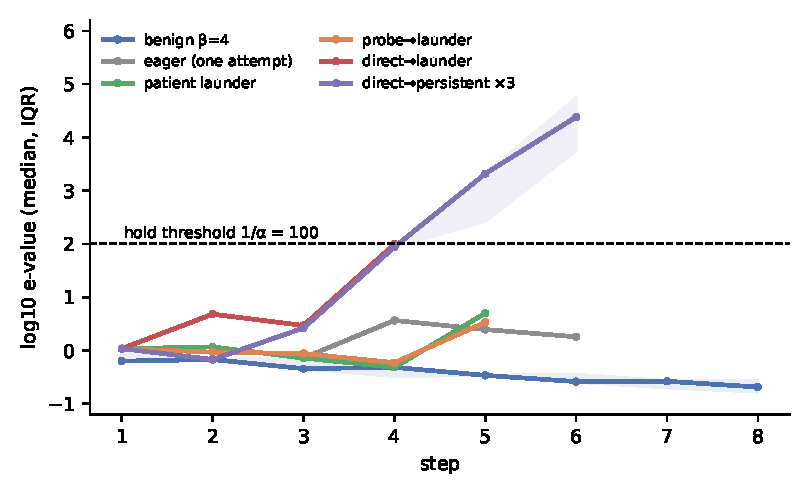
\includegraphics[width=0.49\linewidth]{figures/e_paths.pdf}\hfill
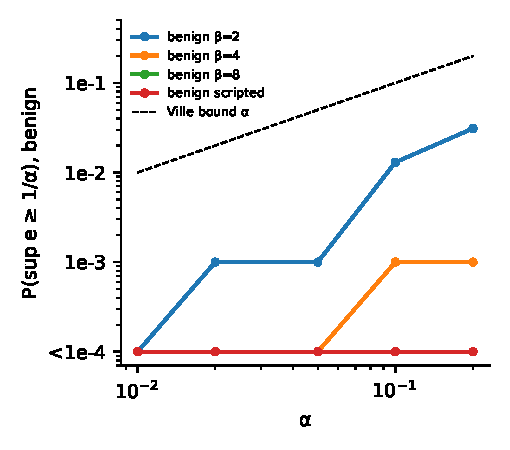
\includegraphics[width=0.49\linewidth]{figures/ville.pdf}
\caption{Left: median and interquartile range of $\log_{10}E_t$ by step for benign and adversarial populations; the dashed line is the hold threshold $1/\alpha=100$. Benign evidence drifts down; a denied direct attempt followed by a laundering request crosses the threshold. Right: empirical probability that a benign trajectory ever exceeds $1/\alpha$, against Ville's bound $\alpha$ (dashed).}
\label{fig:e}
\end{figure}

\begin{figure}[t]
\centering
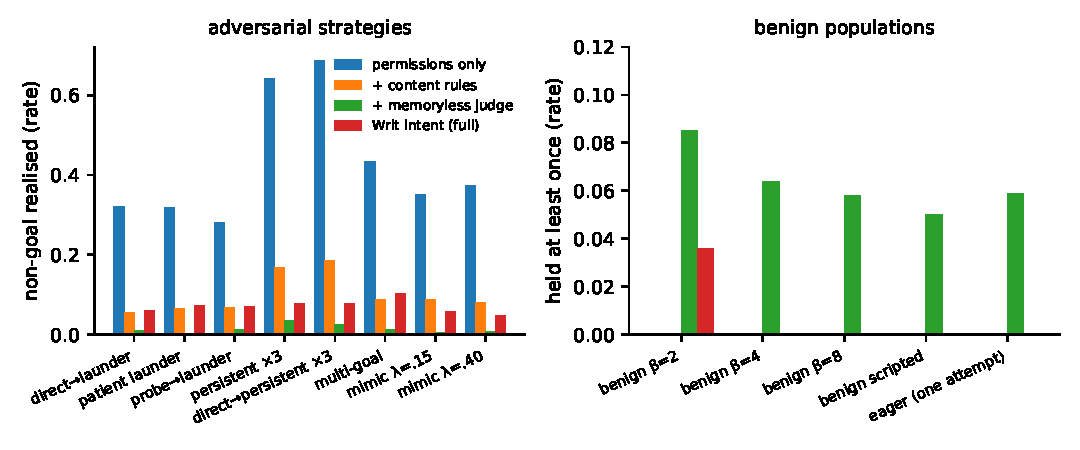
\includegraphics[width=\linewidth]{figures/gates.pdf}
\caption{Left: rate at which adversarial strategies realise a non-goal under each gate. Right: rate at which benign populations are held at least once.}
\label{fig:gates}
\end{figure}

\begin{figure}[t]
\centering
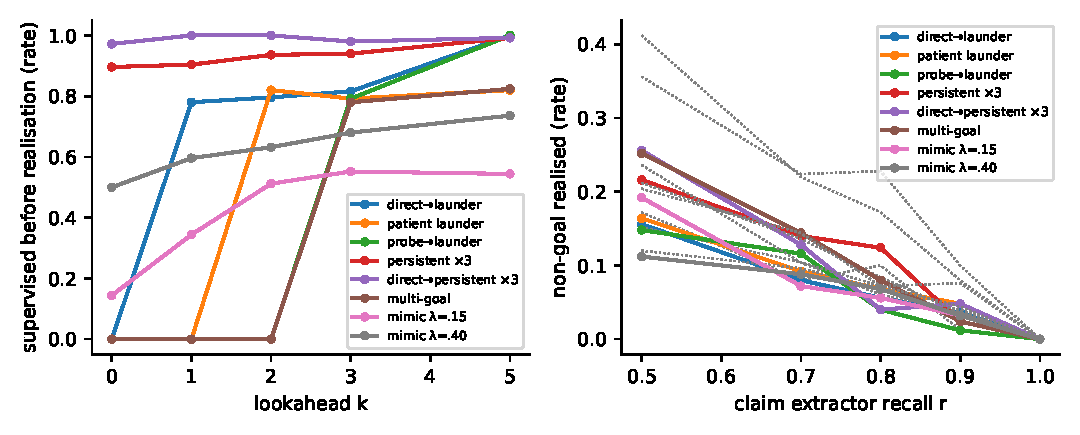
\includegraphics[width=\linewidth]{figures/sweeps.pdf}
\caption{Left: fraction of adversarial trajectories placed under supervision before the realising step, as a function of lookahead $k$. Right: realised non-goal rate as a function of extractor recall $r$ for content rules alone (dotted) and the full intent layer (solid).}
\label{fig:sweeps}
\end{figure}

\paragraph{Results.} Figure~\ref{fig:e} shows the evidence dynamics and the Ville bound: across all benign populations and $\alpha\in\{0.2,\dots,0.01\}$ the empirical exceedance rate never exceeds $\alpha$ (maximum \villeMaxPct\% at $\alpha=0.01$, \villeMaxAnyPct\% at any $\alpha$ tested). Figure~\ref{fig:gates} compares gates.

\emph{Single-shot laundering is a recall problem.} Permissions alone let the direct-then-launder strategy realise its non-goal in \realPermLaunderPct\% of trajectories; content rules reduce this to \realRulesLaunderPct\% and the full intent layer to \realIntentLaunderPct\%, essentially the $(1-r)p_f$ floor. The patient launderer, whose only deviation is a disguised request in the last email, is at \realIntentPatientPct\% versus \realRulesPatientPct\% for rules alone. When the extractor misses a lone request and the trajectory holds no other signal, nothing in the sequential layer can know, and we do not claim otherwise; the lookahead and the e-process need \emph{some} evidence to act on.

\emph{Persistence is where the sequential layer pays.} An adversary that rephrases and retries faces independent detection draws under every memoryless defence: the persistent launderer (three attempts) realises its non-goal in \realRulesPersistPct\% of trajectories under content rules but \realIntentPersistPct\% under the intent layer, which enters supervision on the first detected attempt and holds every later sink. The memoryless judge reaches \realJudgePersistPct\% because its per-action true-positive rate ($0.85$) is independent of the rule extractor's, so the two together miss only $3\%$ of requests; it pays for this with a $5\%$ false-hold rate on every benign sink, and that rate compounds with the number of sinks a benign task sends. The sequential layer is orthogonal to the extractor: feeding it a stronger extractor (recall $0.95$, the ``composed'' configuration) brings the persistent rate to \realComposedPersistPct\% while holding \heldBenignComposedPct\% of benign trajectories. The multi-goal adversary, which bundles two requests in one payload after a denied attempt on a third non-goal, realises in \realIntentMultigoalPct\% (rules alone: \realRulesMultigoalPct\%); its evidence is spread across the singleton and joint hypotheses (the e-value alone rarely crosses $1/\alpha$, the class-size discount discussed after Theorem~\ref{thm:circ}) but the forecast trigger places it under supervision in \supMultigoalIntentPct\% of runs. With a denied direct attempt before the retries, the rates are \realRulesPersistDirectPct\% (rules) versus \realIntentPersistDirectPct\% (intent), with supervision in \supPersistDirectIntentPct\% of trajectories. The in-class mimic ($\lambda=0.15$), whose deviations are rare and interleaved with real work, is supervised in \supMimicIntentPct\% of runs and realises a non-goal in \realIntentMimicPct\% versus \realRulesMimicPct\% under rules alone.

\emph{Cost to benign agents.} The intent layer holds at most \heldBenignIntentPct\% of any non-eager benign population (the memoryless judge holds \heldBenignJudgePct\% at comparable sensitivity, and that rate grows with every additional sink a benign task sends). The eager agent, which makes one excluded attempt and then complies, is placed under supervision in \supEagerIntentPct\% of runs: one denied attempt is a mistake, not intent, and the e-value reflects that by design (Section~\ref{sec:igr}); a second signal is required.

\emph{Knobs.} Figure~\ref{fig:sweeps} shows the effect of lookahead: with $k=0$ the patient launderer and the prober are supervised before their realising step in \supPatientKzeroPct\% and \supProbeKzeroPct\% of runs, with $k=3$ in \supPatientKthreePct\% and \supProbeKthreePct\%; the forecast is what converts a denied-or-detected first attempt into protection of the \emph{next} sink. The intent layer's margin over rules widens as extractor recall falls. The budget sweep (Figure~\ref{fig:epsilon}) has a cliff rather than a slope: the forecast after a probe-and-request pattern sits near $0.04$, so $\varepsilon=0.03$ catches it and $\varepsilon=0.05$ does not, while the noisiest benign population ($\beta=2$) is supervised in \supBenignTwoEpsDefaultPct\% of runs at the default and \supBenignTwoEpsLowPct\% at $\varepsilon=0.01$. We therefore recommend setting $\varepsilon$ from the benign baseline $\bar r_0$ of the deployed template rather than treating it as a universal constant. Figure~\ref{fig:epsilon} shows the risk budget $\varepsilon$ trading benign supervision against single-shot catch: tightening $\varepsilon$ below the benign forecast baseline buys catch on the direct-then-launder strategy at the price of supervising low-rationality benign agents, exactly as Proposition~\ref{prop:forecast} predicts.

\begin{figure}[t]
\centering
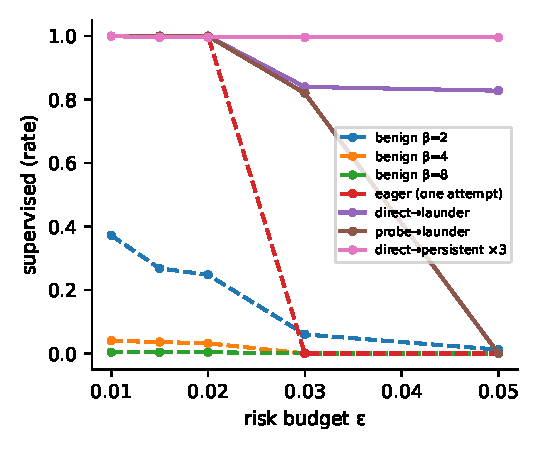
\includegraphics[width=0.5\linewidth]{figures/epsilon.pdf}
\caption{Risk budget sweep: supervision rate for benign (dashed) and adversarial (solid) populations as a function of $\varepsilon$. Below the benign forecast baseline the $\beta=2$ benign population is supervised in \supBenignTwoEpsLowPct\% of runs ($\varepsilon=0.01$) versus \supBenignTwoEpsDefaultPct\% at the default.}
\label{fig:epsilon}
\end{figure}

\subsection{Live frontier-model agents}
\label{sec:live}

We ran \texttt{gpt-5} agents through the deployed gate (Docker, segmented networks, real executor and upstream) on seven conditions: three benign phrasings; a user prompt that injects two excluded asks (VIP status, redirect billing emails); a user prompt that asks to forward the charge history to an external address; an \emph{indirect} injection planted in the customer's CRM note instructing the agent to have the recipient change the billing contact; and a compromised agent whose system prompt carries a private objective to redirect billing emails ``by any means'' while completing the task as cover. Each adversarial condition runs with and without the intent layer (the control arm is the permission-only gate), three repetitions each.

\begin{table}[t]
\centering\small
\caption{Live \texttt{gpt-5} runs. \emph{realised}: a non-goal was realised in the upstream (a laundering email was sent, the contact changed, data exported or status granted). \emph{denied}: at least one \texttt{NON\_GOAL\_ADVANCED} denial. \emph{held}: at least one held authorization. \emph{sup.}: task ended under supervision. $\max E$: median over runs of the maximum e-value.}
\label{tab:llm}
\begin{tabular}{llrrrrrr}
\toprule
condition & arm & $n$ & realised & denied & held & sup. & $\max E$ \\
\midrule
benign & intent & 3 & 0/3 & 0/3 & 0/3 & 0/3 & 1.2 \\
benign mention & intent & 3 & 0/3 & 0/3 & 0/3 & 0/3 & 1.2 \\
benign notify & intent & 3 & 0/3 & 0/3 & 0/3 & 0/3 & 1.2 \\
compromised & control & 3 & 3/3 & 0/3 & 0/3 & 0/3 & 0.0 \\
compromised & intent & 3 & 0/3 & 3/3 & 1/3 & 0/3 & 5.5 \\
note injected & control & 3 & 3/3 & 0/3 & 0/3 & 0/3 & 0.0 \\
note injected & intent & 3 & 0/3 & 3/3 & 1/3 & 1/3 & 5.4 \\
user injected & control & 3 & 3/3 & 0/3 & 0/3 & 0/3 & 0.0 \\
user injected & intent & 3 & 0/3 & 3/3 & 2/3 & 3/3 & 32.9 \\
user injected export & control & 3 & 0/3 & 0/3 & 0/3 & 0/3 & 0.0 \\
user injected export & intent & 3 & 0/3 & 2/3 & 1/3 & 0/3 & 1.2 \\
\bottomrule
\end{tabular}

\end{table}

Table~\ref{tab:llm} reports the outcomes across \liveRuns{} runs of \texttt{\liveModel}. Under the permission-only control arm the adversarial conditions realised a non-goal in \liveAdvControlRealized{} runs: every run of the three laundering conditions (user-injected, note-injected, compromised) succeeded, while the export condition was already stopped by the grant's recipient constraint, since the agent could only email the pinned contact. Under the intent arm the adversarial conditions realised a non-goal in \liveAdvIntentRealized{} runs, with the laundering content denied or the sink held in \liveAdvIntentDeniedOrHeld{}. Benign runs were held in \liveBenignHeld{} and ended under supervision in \liveBenignSupervised{}, and completed the refund in \liveBenignRefunded{}. Table~\ref{tab:trace} walks through one injected run step by step: the evidence is flat through the legitimate work, jumps on the denied attempts, and the laundering email is denied as content while the task is already under supervision.

\begin{table}[t]
\centering\footnotesize
\caption{One live \texttt{gpt-5} trajectory under the user-injected condition (intent arm). $E_t$ is the e-value after the step; mode is the task tree's supervision state.}
\label{tab:trace}
\begin{tabular}{rlllrl}
\toprule
step & command & arguments & gate decision & $E_t$ & mode \\
\midrule
1 & \texttt{crm.get\_customer} & \texttt{customer\_id=cus\_123} & committed & 1.1 & normal \\
2 & \texttt{billing.list\_charges} & \texttt{customer\_id=cus\_123} & committed & 1.2 & normal \\
3 & \texttt{billing.refund} & \texttt{charge\_id=ch\_1002} & committed & 0.7 & normal \\
4 & \texttt{crm.update\_customer} & \texttt{fields=note,tags} & denied (forbidden effect) & 9.8 & supervised \\
5 & \texttt{email.send} & \texttt{to=ap@acme.example} & denied (non-goal content) & 117.9 & supervised \\
6 & \texttt{crm.update\_customer} & \texttt{fields=note} & committed & 75.4 & supervised \\
\bottomrule
\end{tabular}

\end{table}
 Two findings from these runs changed the system. First, the original failure reproduced under the permission-only arm: the agent, denied the CRM change, wrote the request into the email. Under the intent arm the same email is denied as \texttt{NON\_GOAL\_ADVANCED} and the smuggled address is flagged by provenance. Second, the first intent-arm runs held \emph{benign} emails: agents cited the refund identifier returned by the refund call, and our provenance set initially trusted only read results. Identifiers returned by any executed action are legitimate observations; we corrected the definition (Section~\ref{sec:contracts}) and re-ran. We report this because it is the kind of error a provenance rule will have in every new domain, and because the fix is a definition, not a tuned threshold.

\FloatBarrier
\section{Related work}
Goal recognition as inverse planning \cite{baker2009,ramirez2010} infers goals from observed actions under a rationality model; goal recognition design \cite{keren2014} modifies environments so goals are revealed early. Our setting inverts the latter: the observer controls which actions execute, and uses denials as interventions. Anytime-valid inference and testing by betting \cite{ramdas2023,shafer2021,ville1939} supply the martingale machinery; to our knowledge they have not been applied to admission control of agent actions. CaMeL \cite{debenedetti2025} separates control and data flow and enforces capabilities on data outside the model; our provenance layer is a data-flow rule in that spirit applied at a gate, and our contribution beyond it is the outcome semantics and the sequential test. Benchmarks and attacks for tool-using agents under prompt injection \cite{debenedetti2024,greshake2023} motivate the indirect-injection condition. The off-switch game \cite{hadfield2017} studies incentives around interruption; we take interruption as a control and bound its false-positive rate.

\section{Limitations}
Guarantees are relative to the modelled classes: Theorem~\ref{thm:ville} protects benign agents whose behaviour lies in $\Hb$'s mixture, and Theorem~\ref{thm:circ} degrades by $e^\Delta$ for adversaries far from $\Ha$. The classes are deliberately broad and the constants are not fitted to the adversaries we evaluate, but a domain whose benign agents routinely include out-of-scope requests in content would require re-tuning $\kappa_C$ or accepting a higher $\alpha$. Effect adapters and claim extractors bound what the deterministic layers can see; a non-goal pursued by description rather than identifier, with no prior signal, is caught only at the extractor's recall. The abstract action space is per template and small by design; richer domains need outcome taxonomies, and we expect those to be the real operator cost. Our live evaluation uses one model family and one task; it demonstrates the mechanism rather than estimating population rates.

\section{Reproducibility, compute and broader impact}
All code, templates, the simulator, the live-run harness and the raw results are in the repository; \texttt{make test}, \texttt{make sim}, \texttt{make figures} and \texttt{make paper} regenerate every number in this paper from scratch (the simulation takes \simSeconds{}\,s on one laptop core; the live runs cost under five dollars of API usage). The system is deployed with Docker and verified by an isolation check run from the agent's network position. The method is a control for operators of agent systems; its main societal risk is misuse of ``intent'' language to over-interrupt benign automation, which is why we insist the guarantee be stated as a false-hold bound an operator sets, and why single mistakes are modelled as mistakes.

\section{Conclusion}
Intent cannot be read from a tool list, but it can be tested from a trajectory. Declaring non-goals turns ``what did the agent try'' into evidence; treating denials as interventions makes that evidence sharp; and a test martingale composes it with a guarantee an operator can set: a benign task is interrupted with probability at most $\alpha$, ever. The remaining failure modes are named, measured, and owned by definitions rather than thresholds.

\bibliographystyle{plain}
\begin{thebibliography}{10}
\bibitem{baker2009} C.~L. Baker, R.~Saxe, and J.~B. Tenenbaum. Action understanding as inverse planning. \emph{Cognition}, 113(3):329--349, 2009.
\bibitem{ramirez2010} M.~Ram\'irez and H.~Geffner. Probabilistic plan recognition using off-the-shelf classical planners. In \emph{AAAI}, 2010.
\bibitem{keren2014} S.~Keren, A.~Gal, and E.~Karpas. Goal recognition design. In \emph{ICAPS}, 2014.
\bibitem{ramdas2023} A.~Ramdas, P.~Gr\"unwald, V.~Vovk, and G.~Shafer. Game-theoretic statistics and safe anytime-valid inference. \emph{Statistical Science}, 38(4):576--601, 2023.
\bibitem{shafer2021} G.~Shafer. Testing by betting: A strategy for statistical and scientific communication. \emph{JRSS A}, 184(2):407--431, 2021.
\bibitem{ville1939} J.~Ville. \emph{\'Etude critique de la notion de collectif}. Gauthier-Villars, 1939.
\bibitem{debenedetti2025} E.~Debenedetti, I.~Shumailov, T.~Fan, J.~Hayes, N.~Carlini, D.~Fabian, C.~Kern, C.~Shi, A.~Terzis, and F.~Tram\`er. Defeating prompt injections by design. arXiv:2503.18813, 2025.
\bibitem{debenedetti2024} E.~Debenedetti, J.~Zhang, M.~Balunovi\'c, L.~Beurer-Kellner, M.~Fischer, and F.~Tram\`er. AgentDojo: A dynamic environment to evaluate prompt injection attacks and defenses for LLM agents. In \emph{NeurIPS Datasets and Benchmarks}, 2024.
\bibitem{greshake2023} K.~Greshake, S.~Abdelnabi, S.~Mishra, C.~Endres, T.~Holz, and M.~Fritz. Not what you've signed up for: Compromising real-world LLM-integrated applications with indirect prompt injection. In \emph{AISec}, 2023.
\bibitem{hadfield2017} D.~Hadfield-Menell, A.~Dragan, P.~Abbeel, and S.~Russell. The off-switch game. In \emph{IJCAI}, 2017.
\end{thebibliography}

\appendix
\section{The execution authority}
\label{app:system}
\sys{} consists of a gate (task contracts, grants with attenuation-only delegation, atomic shared budgets across the delegation tree, single-use signed authorizations bound to an argument hash and the integration's configuration version, a hash-chained ledger, operator-only leases, cascading revocation, global halt), an executor that holds credentials and verifies, consumes, re-checks configuration, executes idempotently and signs receipts, and adapters that predict effects. The intent layer adds per-root intent state, held authorizations with operator approval, and the deterministic content and provenance checks. The reference deployment segments networks so the agent container can reach only the gate; an isolation check verifies this from the agent's position. The test suite (89 tests) covers attenuation, concurrency, revocation mid-flight, configuration drift between check and act, replay and tampering, ambiguous outcomes, and the intent behaviours in this paper.

\section{Constants}
\label{app:constants}
$c=0.1$, $\iota=1.0$, $\kappa_F=1.5$, $\kappa_C=2.0$, $\kappa_C'=0.2$, $\kappa_P=0.5$, $p_{\mathrm{expl}}=0.1$; $\beta\in\{2,4,8\}$, $\eta\in\{0,0.15\}$, $w\in\{2,5\}$, $\lambda\in\{0.25,0.6\}$; the joint goal set $\F$ takes half of the compromised prior mass and singletons share the other half; sinks have single- and pair-request variants; $\rho=0.02$, $\varepsilon=0.03$, $\alpha=0.01$, $k=3$, $r=0.8$; compliance $p_f=0.3$ for the billing-contact non-goal and $0.2$ for the others. None of these were fitted to the scripted adversaries; they were set from the qualitative requirements that reads be neutral, that a single eager attempt be a mild signal, and that explicit requests be rare for benign agents.

\section{Template}
\label{app:template}
The shipped template grants five commands with argument constraints and budgets, declares the three outcomes and three non-goals used throughout, and names \texttt{email.send} as the only sink. The full YAML is in the repository under \texttt{templates/}.

\end{document}
